\documentclass[11pt,a4paper]{article}

% ============================================================
% PAQUETES
% ============================================================
\usepackage[utf8]{inputenc}
\usepackage[T1]{fontenc}
\usepackage{lmodern}          % fuentes vectoriales (evita Type 3 de mapa de bits)
\usepackage[spanish,es-noshorthands]{babel}
\usepackage{microtype}
\usepackage{geometry}
\geometry{a4paper,margin=2.3cm}
\usepackage{booktabs}
\usepackage{array}
\usepackage{longtable}
\usepackage{graphicx}
\usepackage{caption}
\usepackage{subcaption}
\usepackage{fancyhdr}
\usepackage{xcolor}
\usepackage{xurl}
\usepackage{hyperref}
\usepackage{enumitem}
\usepackage{natbib}
\usepackage{amsmath}
\usepackage{tikz}
\usetikzlibrary{arrows.meta,positioning}

\hypersetup{
  colorlinks=true,
  linkcolor=blue!50!black,
  urlcolor=blue!60!black,
  citecolor=blue!50!black,
  pdftitle={Entregable 1 -- Influencia del cambio climático en los eventos de El Niño y sus impactos en el Perú},
  pdfauthor={Jonathan Aaron Paredes Quispe}
}

% Esta instalacion de TeX no trae patrones de guionado en espanol
% (paquete texlive-lang-spanish): se desactiva el guionado automatico
% para no cortar palabras con reglas del ingles. microtype y
% \emergencystretch compensan el espaciado.
\hyphenpenalty=10000
\exhyphenpenalty=10000
\setlength{\emergencystretch}{3em}

% Rutas y nombres de archivo en monoespaciada, con corte de linea
% permitido y en color de texto normal.
\urlstyle{tt}
\newcommand{\archivo}[1]{\begingroup\hypersetup{urlcolor=black}\url{#1}\endgroup}
\newcolumntype{L}[1]{>{\raggedright\arraybackslash}p{#1}}

% Macros compartidas entre el informe revisado y las auditorias.
% Cifras verificadas contra los archivos del repositorio (ver A01/A04/A07):
\newcommand{\nUniverso}{102}   % source_id CMIP6 con tos/Omon en ESGF (00b, model_availability_priority.csv)
\newcommand{\nSeed}{41}        % publican los cuatro experimentos (config/models_seed_cmip6.csv)
\newcommand{\nSel}{40}         % completos + QC PASS (models_inventory_final.csv)
\newcommand{\nComb}{160}       % combinaciones modelo-experimento PASS (qc_report.csv)
\newcommand{\nNoEnc}{44}       % config/models_no_encontrado_44.csv
\newcommand{\nParcial}{18}     % 102 - 40 - 44
% Fecha de la portada: fija (no \today), editable en un solo lugar.
\newcommand{\fechaentrega}{28 de septiembre de 2026}
% Estado de codigo que documenta el E1 (antes de los cambios del E2)
\newcommand{\commitEone}{\texttt{8ee6184}}

\graphicspath{{../}}

\pagestyle{fancy}
\fancyhf{}
\fancyhead[L]{\small Entregable N.\textsuperscript{o}~1 -- Influencia del cambio climático en los eventos de El Niño y sus impactos en el Perú}
\fancyhead[R]{\small \thepage}
\renewcommand{\headrulewidth}{0.4pt}
\setlength{\headheight}{14pt}

\setlength{\parskip}{0.4em}
\setlength{\parindent}{1.2em}

\begin{document}

% ============================================================
% PORTADA (formato de tapa de los entregables)
% ============================================================
\pagenumbering{Alph}
\begin{titlepage}
\centering
\noindent\rule{\textwidth}{0.6pt}

\vspace{1.2cm}
{\Large \bfseries ENTREGABLE N.\textsuperscript{o}~1 \par}
\vspace{1.2cm}
\rule{0.7\textwidth}{0.6pt}

\vspace{1.2cm}
{\normalsize \bfseries Concepto: \par}
\vspace{0.3cm}
{\large \bfseries Servicio de asistencia en temas de investigación para evaluar\\
la influencia del cambio climático en los eventos de El Niño\\
y sus impactos en el Perú \par}

\vspace{1.4cm}
{\small Prestado para: Servicio Nacional de Meteorología e Hidrología del Perú -- SENAMHI \par}

\vspace{1.4cm}
{\normalsize \bfseries Actividad: \par}
\vspace{0.2cm}
{\normalsize Primer entregable -- Informe de la actividad a)\\
del numeral 6 de los términos de referencia \par}

\vspace{1.2cm}
\rule{0.7\textwidth}{0.6pt}

\vspace{0.3cm}
{\small \bfseries Responsable: \par}
\vspace{0.2cm}
{\small Ing. Jonathan Aaron Paredes Quispe \par}
\vspace{0.3cm}
\rule{0.7\textwidth}{0.6pt}

\vfill
{\small \bfseries FECHA: \fechaentrega \par}
\vspace{0.6cm}
\noindent\rule{\textwidth}{0.6pt}
\end{titlepage}

\pagenumbering{roman}
\tableofcontents
\clearpage
\listoffigures
\listoftables
\clearpage
\pagenumbering{arabic}

% ============================================================
\section{Resumen}
\label{sec:resumen}
% ============================================================

Este informe documenta el Entregable~1 del servicio de asistencia en temas de investigación del SENAMHI orientado a evaluar la influencia del cambio climático sobre El Niño-Oscilación del Sur (ENOS) en las regiones oceanográficas Niño~3.4 y Niño~1+2. En cumplimiento de la actividad~(a) de los términos de referencia, el entregable cubre la revisión de metodologías de tiempo de emergencia (TOE, por sus siglas en inglés), la recopilación de la temperatura superficial del mar (TSM) observada y la recopilación de las simulaciones históricas y futuras de los modelos CMIP6. No produce todavía resultados de desempeño, proyección ni TOE, que corresponden a los Entregables~2 a~4, pero deja construido, verificado y versionado el insumo del que esos entregables dependen.

El producto operativo es un \emph{pipeline} reproducible (repositorio \archivo{smn_toe}, con un único punto de entrada, \texttt{run.sh}) que descarga, homogeneiza, enmascara y valida la variable \texttt{tos} (TSM, tabla CMOR \texttt{Omon}) de los modelos CMIP6 que publican los experimentos \texttt{historical}, \texttt{ssp245} y \texttt{ssp585}, más \texttt{ssp370} como escenario intermedio adicional, junto con la referencia observacional ERSSTv5 de NOAA. El universo de partida son los 102 modelos CMIP6 que publican \texttt{tos}/\texttt{Omon} en la federación ESGF; 41 de ellos publican los cuatro experimentos y 40 completaron la descarga y aprobaron el control de calidad (160 combinaciones modelo-experimento, Sección~\ref{sec:resultados}). Los 62 restantes quedaron excluidos por no publicar alguno de los experimentos en ninguna fuente consultada (44) o por disponibilidad o descarga incompleta (18).

El \emph{pipeline} incorpora controles específicos frente a problemas que contaminarían el dato sin producir errores visibles. Cuatro provienen de los datos y servicios de origen: valores de relleno que el regrillado no reconoce como faltantes (FGOALS-f3-L), filtrados por valor físico; archivos que declaran grados Celsius pero contienen valores en Kelvin (GISS-E2-1-G), detectados por el valor numérico; búsquedas paginadas en ESGF que un corte de red puede truncar sin aviso, que se repiten completas; y archivos de dos variantes de grilla en un mismo modelo, que se filtran por grilla. Además, el inventario exige explícitamente los cuatro experimentos y el control de calidad se recalcula en cada corrida. El detalle de cada control está en el documento de anexos.

En paralelo, el informe desarrolla la revisión científica: la partición de incertidumbre de \citet{hawkins2012}, su adaptación por \citet{szabo2016}, la aplicación a CMIP6 y Sudamérica de \citet{bruno2023}, el precedente institucional de \citet{alvarez2024}, la caracterización del Niño costero de \citet{takahashi2019} y un estado del arte de otras metodologías de TOE. De esa revisión se deriva la elección de los dos métodos de TOE que se aplicarán en el Entregable~4: M1 \citep{szabo2016} y \emph{Time of Detection} (ToD, \citealp{gopika2024}). Las instrucciones de instalación y uso del \emph{pipeline}, así como la descripción detallada de cada paso, se entregan en un documento de anexos separado.

% ============================================================
\section{Alcance}
\label{sec:alcance}
% ============================================================

Los términos de referencia del \emph{Servicio de asistencia en temas de investigación para evaluar la influencia del cambio climático en los eventos de El Niño y sus impactos en el Perú} (en adelante, TdR) definen el primer entregable, con plazo máximo de 25 días calendario, como el informe de la actividad~(a) del numeral~6: ``Realizar la revisión de metodologías sobre tiempo de emergencia (TOE), recopilación de datos de la información de temperatura superficial del mar (TSM), y simulaciones históricas y futuras de los modelos climáticos globales CMIP6 para los escenarios SSP2-4.5 y SSP5-8.5, correspondientes a las regiones Niño~3.4 y Niño~1+2''.

Para operacionalizar este mandato, el equipo técnico lo descompone en cinco tareas: (i) revisar los antecedentes científicos (ENOS y Niño costero, partición de incertidumbre, aplicaciones previas en Sudamérica y otras metodologías de TOE); (ii) consolidar el conjunto de modelos CMIP6 que publican la variable requerida; (iii) recopilar la referencia observacional ERSSTv5; (iv) definir los dominios oceanográficos y los periodos de análisis; y (v) homogeneizar unidades, calendarios, resoluciones espaciales y máscaras océano-tierra entre todas las fuentes. La tarea~(i) es de revisión bibliográfica y se desarrolla en la Sección~\ref{sec:marco}; las tareas (ii) a (v) son computacionales y se resuelven con el \emph{pipeline} descrito en las Secciones~\ref{sec:datos} a~\ref{sec:scripts}.

El control de calidad de este entregable verifica que el dato esté completo y homogéneo, no que los modelos representen bien el clima observado: esa evaluación de desempeño es materia del Entregable~2.

% ============================================================
\section{Revisión científica}
\label{sec:marco}
% ============================================================

\subsection{Antecedentes}
\label{sec:antecedentes}

\textbf{Partición de incertidumbre (Hawkins y Sutton).} \citet{hawkins2009,hawkins2011precip} establecieron la partición de la incertidumbre de una proyección climática en tres fuentes: variabilidad interna ($V$, no reducible, propia de la dinámica caótica del sistema climático), incertidumbre de modelo ($M$, dispersión entre las respuestas de distintos modelos ante un mismo forzante) e incertidumbre de escenario ($S$, dispersión entre trayectorias de emisiones). Cada simulación se ajusta con un polinomio de cuarto orden, el residuo del ajuste representa la variabilidad interna y, al tratar las tres fuentes como independientes, la varianza total es su suma, $T = V + M + S$. \citet{hawkins2012} llevaron el marco al \emph{Time of Emergence} por modelo individual: la señal local se obtiene regresando la variable sobre la temperatura media global suavizada con el mismo polinomio, el ruido es la desviación estándar interanual del residuo y el TOE es el primer año en que la razón señal-ruido supera 1 o 2. Estimaron además que la incertidumbre del propio TOE es de al menos 30 años y llega a 60 en algunas regiones. La partición en tres fuentes es la base del análisis de incertidumbre previsto en el TdR para el Entregable~4.

\textbf{Aplicación de Szabó y Szépszó.} \citet{szabo2016} implementan el método de Hawkins y Sutton para temperatura y precipitación sobre Europa (15 modelos CMIP3, tres escenarios SRES, referencia 1971--2000) e introducen cuatro cambios: la variabilidad interna se recalcula cada año sobre los 30 años previos, en lugar de asumirse constante; se usan medias anuales y estacionales en vez de decadales; los modelos no se ponderan; y el TOE se define con la variabilidad interna como único ruido, mientras que la razón señal-ruido conserva la incertidumbre total. Esta formulación es la que el equipo técnico adopta como método M1 (Sección~\ref{sec:toe_metodos}).

\textbf{Trabajo de Bruno Ramírez.} \citet{bruno2023}, trabajo de suficiencia profesional de la Universidad Nacional Agraria La Molina, aplica la metodología de \citet{szabo2016} a temperatura y precipitación sobre Sudamérica con 53 modelos CMIP6, periodo de referencia 1981--2010 (1981--2014 en este proyecto) y los escenarios SSP2-4.5 y SSP5-8.5, calculando variabilidad interna, razón señal-ruido y TOE. Su validación de modelos combina un componente físico (posición e intensidad del anticiclón del Pacífico Sur, la Alta de Bolivia y la Baja Amazónica) y uno estadístico frente a ERA5 (correlación de Pearson, sesgo, RMSE y diagrama de Taylor). Es el antecedente metodológico más cercano: muestra que M1 ya se aplicó con CMIP6 en Sudamérica, aunque sobre variables atmosféricas continentales y no sobre las cajas oceánicas Niño~3.4 y Niño~1+2. Su lista de modelos se tomó como referencia para la selección de este entregable, que abarca todo el catálogo CMIP6 disponible (Sección~\ref{sec:desviacion}).

\textbf{Trabajo de Álvarez Sánchez.} \citet{alvarez2024}, también trabajo de suficiencia profesional de la misma universidad, proyectó la temperatura superficial del mar y el nivel del mar en las costas de Sudamérica y el Pacífico tropical con modelos CMIP5. Comparte con este proyecto el dominio oceánico y permite, en entregables posteriores, contrastar las generaciones CMIP5 y CMIP6.

\textbf{Niño costero.} \citet{takahashi2019} reconstruyen con observaciones in situ el Niño costero de 1925: calentamiento intenso en el Pacífico oriental lejano con condiciones frías en el Pacífico central, a diferencia de los eventos extraordinarios de 1982--1983 y 1997--1998. Las ondas Kelvin ecuatoriales tuvieron un papel menor en su inicio; el evento se asocia con vientos del norte a través del ecuador, con la intensificación de la zona de convergencia intertropical al sur del ecuador y con realimentaciones océano-atmósfera locales. Existen, por tanto, dos tipos de eventos de fuerte impacto en Niño~1+2, con dinámicas distintas, lo que justifica analizar esta caja por separado de Niño~3.4.

La revisión de metodologías de TOE que pide la actividad~(a) se extendió más allá de Hawkins-Sutton y Szabó; la Sección~\ref{sec:referencias} sintetiza la bibliografía revisada, de la que se deriva el método complementario ToD (Sección~\ref{sec:toe_metodos}).

\subsection{Literatura sobre \emph{Time of Emergence}}
\label{sec:referencias}

El Cuadro~\ref{tab:referencias} resume la bibliografía sobre TOE revisada para este proyecto: los antecedentes de la Sección~\ref{sec:antecedentes} y literatura complementaria que sustenta la discusión del Entregable~4.

\begin{longtable}{@{}L{3.6cm}L{3.2cm}L{\dimexpr\textwidth-3.6cm-3.2cm-4\tabcolsep\relax}@{}}
\caption{Bibliografía sobre \emph{Time of Emergence} revisada para este proyecto.}
\label{tab:referencias} \\
\toprule
\textbf{Referencia} & \textbf{Dominio} & \textbf{Aporte principal a este proyecto} \\
\midrule
\endfirsthead
\toprule
\textbf{Referencia} & \textbf{Dominio} & \textbf{Aporte principal a este proyecto} \\
\midrule
\endhead
\citet{hawkins2009,hawkins2011precip} & Global y regional (CMIP3) & Partición de la incertidumbre en tres fuentes ($T=V+M+S$) \\
\citet{hawkins2012} & Global, temperatura del aire (CMIP3) & TOE por modelo individual; umbrales S/N de 1 y 2 \\
\citet{szabo2016} & Europa (CMIP3) & Método M1: variabilidad interna móvil; TOE con ruido igual a $V$ \\
\citet{bruno2023} & Sudamérica, temperatura y precipitación (CMIP6) & Aplicación de M1 a CMIP6 en Sudamérica \\
\citet{alvarez2024} & Costas de Sudamérica y Pacífico tropical (CMIP5) & Antecedente institucional; comparación CMIP5 frente a CMIP6 \\
\citet{takahashi2019} & Pacífico oriental lejano & Dinámica del Niño costero \\
\citet{gopika2024} & Océanos tropicales, 30°S--30°N (CMIP5/6) & \emph{Time of Detection} (ToD), método complementario adoptado \\
\citet{zhong2023} & Pacífico tropical (CMIP6 y grandes ensambles) & Regímenes de incertidumbre distintos para el estado medio y para el ENOS \\
\citet{larson2025} & Océano global (CESM2, 1900--2014) & La variabilidad de la circulación forzada por viento retrasa el TOE de la TSM \\
\citet{poul2025} & Mar del Norte, Báltico y Atlántico Norte & Razón S/N con varianzas combinadas; la surgencia retrasa el TOE \\
\citet{keller2014} & Océano global, biogeoquímica (CMIP5) & TOE de TSM de 45--90 años; TOE largo frente a Perú y Chile \\
\citet{chadwick2019} & Chile semiárido y mediterráneo & TOE local por potencia estadística; relación entre CV y TOE \\
\citet{lois2026} & Océano Austral (CMIP6) & \emph{Storylines} y TOE; criterio alternativo de selección de modelos \\
\citet{giorgi2009} & Precipitación global (CMIP3) & TOE de \emph{hot-spots}; emergencia tardía en la cuenca amazónica \\
\citet{john2023,deng2022,barrow2019,ryu2024,ryu2025,im2021,nguyen2018} & Australia, Canadá, Corea del Sur, oeste de EE.\,UU., CORDEX-CORE, precipitación global & Otras aplicaciones de TOE revisadas y no adoptadas (hidrología, extremos de temperatura, estrés térmico, aridez, precipitación) \\
\bottomrule
\end{longtable}

El hallazgo transversal de esta bibliografía es que no existe un método estándar de TOE y que las decisiones metodológicas desplazan la fecha resultante en décadas. El umbral varía entre estudios (S/N de 1 en \citealp{szabo2016}, de 1 y 2 en \citealp{hawkins2012}, de 1{,}6 en \citealp{gopika2024} y de 2 en \citealp{poul2025}); \citet{hawkins2012} estiman una incertidumbre del TOE de 30 a 60 años, y \citet{chadwick2019} encuentran diferencias de más de 40 años según el percentil de tendencia de los modelos. El equipo técnico adopta el método de Szabó (M1) y añade el ToD de Gopika como segundo método independiente, para reportar un rango de fechas y no un único número.

\subsection{Implicancias de la bibliografía para Niño~3.4 y Niño~1+2}
\label{sec:similitudes}

Siete referencias del Cuadro~\ref{tab:referencias} merecen una lectura específica frente al enfoque de este proyecto.

\citet{gopika2024} no solo aportan el método ToD, adoptado como segunda estimación del TOE: analizan 69 simulaciones CMIP5/6 y cuatro productos observacionales en todo el trópico (30°S--30°N) y encuentran que el Pacífico ecuatorial oriental (EEP, por sus siglas en inglés) es la excepción principal. Allí el calentamiento es detectable en más del 90\,\% de los modelos, pero solo en uno de los cuatro productos observacionales, porque los modelos simulan un calentamiento más intenso que el observado. La caja EEP de esta literatura (2{,}5°S--2{,}5°N, 180°--90°O en \citealp{zhong2023}) se superpone a Niño~3.4 y no incluye Niño~1+2. Los mismos autores detectan, en observaciones y en cerca del 80\,\% de los modelos, un calentamiento del Pacífico sudeste más débil que el promedio tropical. Ambos resultados indican que, antes de proyectar, hay que evaluar el sesgo de los modelos en el Pacífico tropical oriental, tarea del Entregable~2.

\citet{zhong2023} establecen una distinción que este proyecto adopta como principio de diseño. Con tres grandes ensambles y CMIP6, muestran que en el EEP la variabilidad interna explica menos de la mitad de la incertidumbre del TOE de la TSM media anual (21\,\% en CESM1-LE), de modo que dominan las diferencias entre modelos. En cambio, explica cerca del 80\,\% de la incertidumbre del TOE de la TSM asociada al ENOS (77\,\% para la precipitación) en CESM1-LE, el único ensamble con suficientes miembros con señal emergente. El estado medio y la variabilidad del ENOS no comparten, por tanto, el mismo régimen de incertidumbre, y deben analizarse por separado en los Entregables~3 y~4.

\citet{larson2025} y \citet{poul2025} documentan, por dos vías distintas, que la dinámica oceánica costera retrasa el TOE de la TSM. En dos ensambles de CESM2 para el periodo histórico (1900--2014), \citet{larson2025} muestran que la variabilidad interna de la circulación forzada por el viento aumenta el ruido y retrasa el TOE en casi todo el océano, más de una década en promedio sobre las latitudes bajas. Además, a lo largo de la frontera oriental del Pacífico, la ausencia de señal emergente coincide con regiones de surgencia forzada por viento. En el Mar del Norte y el Báltico, \citet{poul2025} atribuyen los TOE más tardíos a una surgencia más intensa, que reduce la señal de calentamiento. Frente a Niño~1+2, dominado por la surgencia costera del sistema de la Corriente de Humboldt, ambos resultados apuntan a una emergencia más tardía o más incierta.

\citet{keller2014} reportan, con 17 modelos del sistema terrestre, un TOE de la TSM de 45 a 90 años, mucho mayor que el de las variables biogeoquímicas, e identifican la zona de surgencia de Perú y Chile como una de las regiones con TOE localmente elevado ($>$30 años) para pCO$_2$ y pH. Esta tercera línea, de naturaleza biogeoquímica, es independiente de las anteriores y apunta en el mismo sentido.

\citet{chadwick2019} desarrollan un TOE local para tres cuencas chilenas (Limarí, Maipo y Maule) y concluyen que el TOE de la precipitación es más tardío cuanto mayor es el coeficiente de variación local, con diferencias de más de 40 años según el percentil de tendencia de los modelos. Por analogía, la mayor variabilidad interanual observada en Niño~1+2 anticipa una emergencia más tardía que en Niño~3.4: con ERSSTv5 (1981--2014), la desviación estándar de las anomalías mensuales es de 1{,}08\,°C en Niño~1+2 frente a 0{,}86\,°C en Niño~3.4, y la de las medias anuales, de 0{,}86\,°C frente a 0{,}61\,°C.

\citet{lois2026} aportan un criterio de selección de modelos distinto de la validación física y estadística de \citet{bruno2023}: en lugar de filtrar por desempeño promedio, eligen un subconjunto de modelos CMIP6 que abarca respuestas de circulación y sensibilidades climáticas cualitativamente distintas. Aplicado a este proyecto, el principio sugiere verificar en los próximos entregables que la selección final de modelos no reduzca artificialmente la dispersión de la respuesta de la TSM en ambas cajas, para no subestimar la incertidumbre de modelo ni el rango del TOE en Niño~1+2.

En conjunto, estas líneas de evidencia sustentan una hipótesis de trabajo contrastable en el Entregable~4: \textbf{Niño~1+2 emergerá más tarde, o con mayor incertidumbre, que Niño~3.4}.

\subsection{Elección de los dos métodos de \emph{Time of Emergence}}
\label{sec:toe_metodos}

El TdR prevé para el Entregable~4 el cálculo de la razón señal-ruido y del TOE ``empleando metodologías revisadas''. El equipo técnico adopta como método M1 la formulación de \citet{szabo2016} y la complementa con un segundo método independiente, el \emph{Time of Detection} (ToD) de \citet{gopika2024}. Las ecuaciones se fijan desde este entregable para que el método quede definido antes de calcularlo; el cálculo corresponde al Entregable~4.

\subsubsection{Método M1 (Szabó y Szépszó)}

La señal se estima ajustando un polinomio de cuarto orden a la serie anual o estacional de TSM de cada modelo $m$ y escenario $s$:
\begin{equation}
\label{eq:szabo_signal}
X_{m,s}(t) = \Delta T_{m,s}(t) + \bar{T} + \varepsilon_{m,s}(t),
\end{equation}
donde $\bar{T}$ es el promedio del ajuste en el periodo de referencia (1971--2000 en \citealp{szabo2016}; 1981--2014 en este proyecto, Sección~\ref{sec:dominios_periodos}), $\Delta T_{m,s}(t)$ es la señal de cambio y $\varepsilon_{m,s}(t)$ es el residuo. A diferencia de \citet{hawkins2009}, la variabilidad interna no es constante: es la varianza de los residuos de todos los modelos y escenarios en los 30 años previos, recalculada cada año y suavizada con una media móvil de 10 años:
\begin{equation}
\label{eq:szabo_V}
V(t) = \mathrm{var}_{m,s,\tau}\big(\varepsilon_{m,s}(\tau)\ \big|\ \tau \in [t-29,\,t]\big).
\end{equation}
La incertidumbre de modelo es la varianza entre modelos promediada sobre los escenarios, $M(t)=\frac{1}{N_s}\sum_s \mathrm{var}_m\,\Delta T_{m,s}(t)$; la de escenario es la varianza entre escenarios de la media multimodelo, $S(t)=\mathrm{var}_s\big(\frac{1}{N_m}\sum_m \Delta T_{m,s}(t)\big)$; y, como en \citet{hawkins2009}, la incertidumbre total es su suma:
\begin{equation}
\label{eq:szabo_T}
T(t) = V(t) + M(t) + S(t).
\end{equation}
Con la señal media $G(t)=\frac{1}{N_m N_s}\sum_{m,s}\Delta T_{m,s}(t)$, la razón señal-ruido usa la incertidumbre total, $\mathrm{STN}(t) = G(t)/\sqrt{T(t)}$, mientras que el TOE usa solo la variabilidad interna como ruido:
\begin{equation}
\label{eq:szabo_toe}
\mathrm{TOE} = \min\,\Big\{t : \frac{G(t)}{\sqrt{V(t)}} \geq \kappa\Big\}.
\end{equation}
Se adoptan dos umbrales: $\kappa=1$, el de \citet{szabo2016}, y $\kappa=2$, el umbral más exigente de \citet{hawkins2012}. Separar el ruido de la STN (total) del ruido del TOE (solo interno) es el rasgo distintivo del método. \citet{bruno2023} ya lo aplicó con CMIP6 sobre Sudamérica, con un periodo de referencia similar, lo que reduce el riesgo de implementación.

\subsubsection{Método M2 (ToD, Gopika)}

Como segundo método se adopta el \emph{Time of Detection} de \citet{gopika2024}. En lugar de un umbral fijo de señal-ruido, se evalúa la significancia del coeficiente de una regresión sobre una ventana que crece desde un año inicial $t_0$ hasta $T$:
\begin{equation}
\label{eq:tod}
Y_T(t) = a_T\,W_T(t) + b_T + \varepsilon_T(t), \qquad n_{\text{eff}} = \frac{T-t_0+1}{\sum_{\tau=1}^{n/2} r^2(\tau)},
\end{equation}
donde $Y$ es la TSM de la caja, $W$ es el índice de calentamiento tropical (TSM media 30°S--30°N), $r(\tau)$ es la autocorrelación con desfase $\tau$ y $n_{\text{eff}}$ son los grados de libertad efectivos de la prueba $t$ unilateral sobre $a_T$. El ToD es el último año a partir del cual el coeficiente se vuelve significativo al 95\,\% y se mantiene significativo hasta el final de la serie. No depende de un umbral $\kappa$ sino del nivel de significancia; según los autores, el 95\,\% equivale aproximadamente a una razón señal-ruido de 1{,}6. El índice $W$ requiere la TSM de toda la franja tropical, que queda cubierta por la ventana de descarga del \emph{pipeline} (0°--360°, 30°S--30°N; Sección~\ref{sec:dominios_periodos}).

\begin{table}[htbp]
\caption{Métodos de TOE adoptados.}
\label{tab:metodos_toe}
\small
\begin{tabular}{@{}L{2.3cm}L{5.6cm}L{\dimexpr\textwidth-2.3cm-5.6cm-4\tabcolsep\relax}@{}}
\toprule
\textbf{Método} & \textbf{Ruido de referencia} & \textbf{Criterio de TOE} \\
\midrule
M1 (Szabó) & Variabilidad interna $V(t)$, ventana móvil de 30 años & $G(t)/\sqrt{V(t)} \geq \kappa$, con $\kappa=1$ o $2$ \\
M2 (ToD, Gopika) & Residuo de la regresión, con grados de libertad efectivos & Significancia del coeficiente al 95\,\%, sostenida hasta el final \\
\bottomrule
\end{tabular}
\end{table}

La elección de estos dos métodos responde a tres criterios: (i) M1 cumple directamente lo previsto para el Entregable~4, pues calcula la partición de incertidumbre, la razón señal-ruido y el TOE; (ii) el ToD fue aplicado por \citet{gopika2024} a la TSM tropical, incluido el Pacífico ecuatorial oriental, a diferencia de otros métodos revisados que se aplicaron a ríos australianos \citep{john2023}, a las praderas canadienses \citep{barrow2019} o a Corea del Sur \citep{ryu2024}; y (iii) ambos métodos son conceptualmente independientes (uno se basa en la razón señal-ruido con partición de incertidumbre; el otro, en la significancia estadística de una tendencia), lo que permite reportar un rango de fechas de emergencia en vez de un único número.

% ============================================================
\section{Datos}
\label{sec:datos}
% ============================================================

Se usan dos fuentes. La primera son las salidas de los modelos CMIP6 para la variable \texttt{tos} (TSM, tabla CMOR \texttt{Omon}), obtenidas de la federación ESGF (\emph{Earth System Grid Federation}) y, de forma complementaria, del Copernicus Climate Data Store (CDS). La segunda es ERSSTv5 (\emph{Extended Reconstructed Sea Surface Temperature}, versión~5) de NOAA, descargada de NOAA PSL, que es la referencia observacional única de todo el \emph{pipeline}. La Figura~\ref{fig:cmip6_contribution} muestra la procedencia institucional de los 40 modelos seleccionados.

\begin{figure}[htbp]
\centering
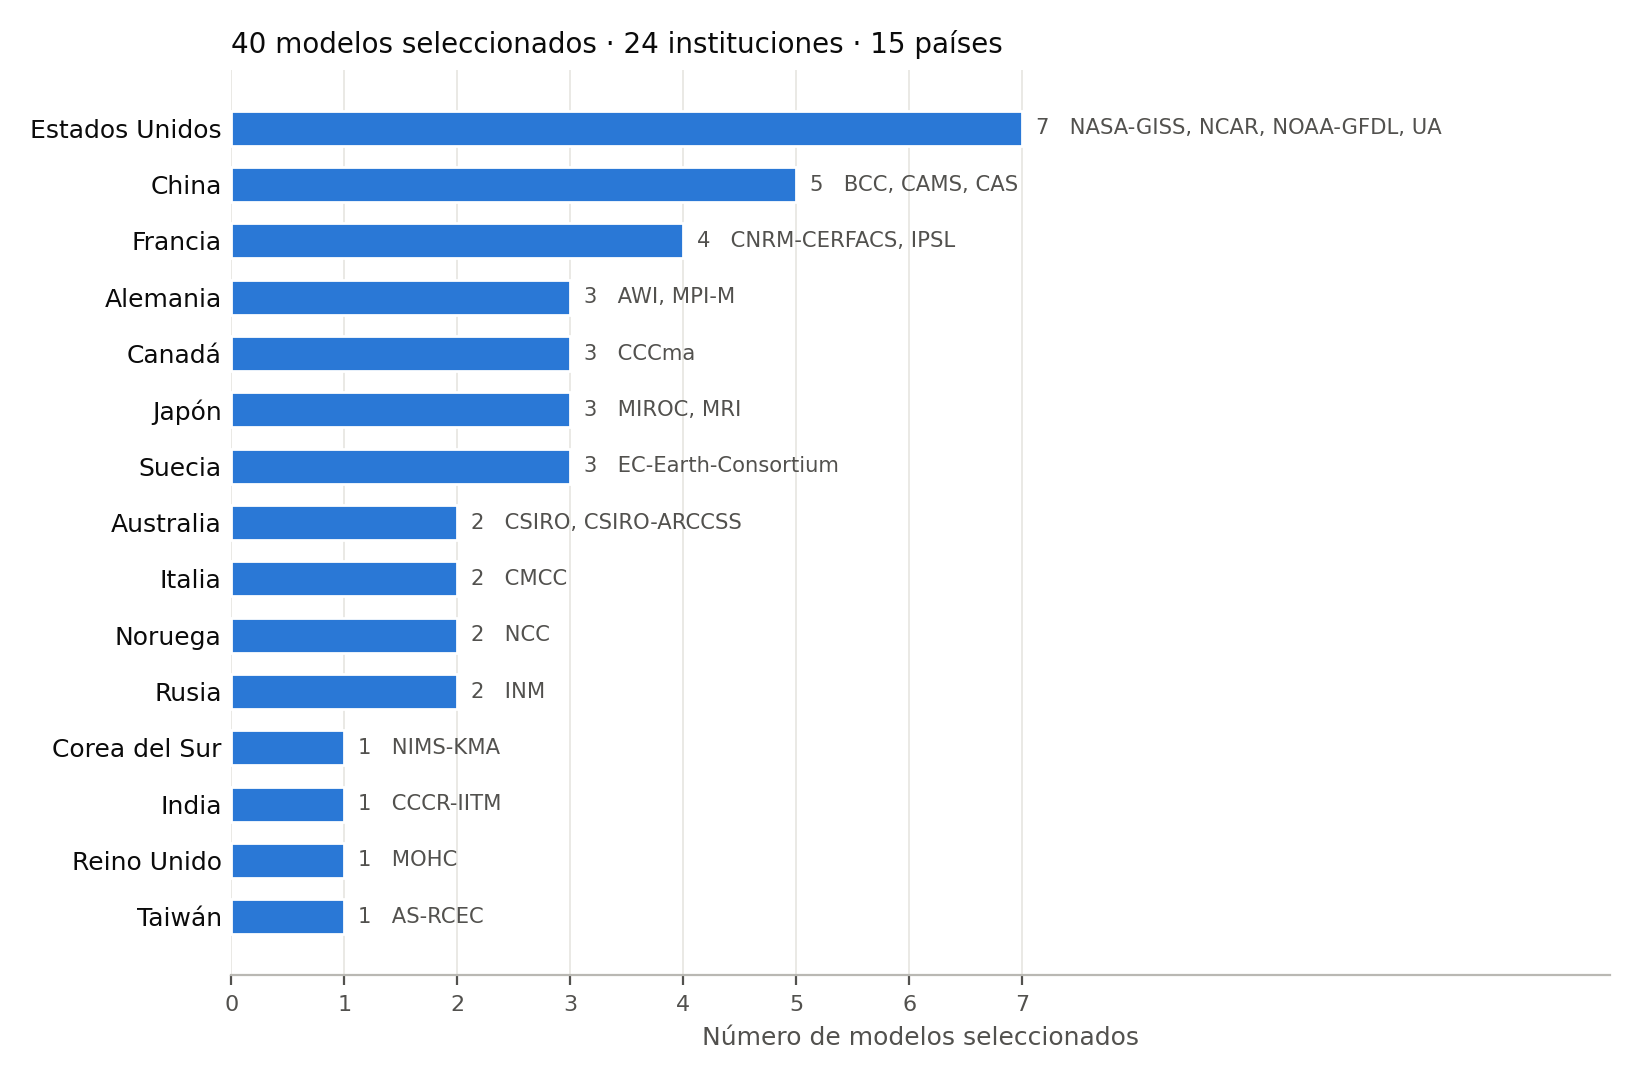
\includegraphics[width=0.92\textwidth]{figuras/contribucion_paises.png}
\caption[Modelos CMIP6 seleccionados por país e institución de origen.]{Modelos CMIP6 seleccionados por país de la institución que los publica, con las instituciones de cada país (fuente: \archivo{informe/model_registry.csv} y \archivo{data/processed/models_inventory_final.csv}). La diversidad de centros de modelado importa para la incertidumbre de modelo: modelos de un mismo centro comparten componentes y, con mayor probabilidad, sesgos estructurales (por ejemplo, la lengua fría o la doble ZCIT del Pacífico oriental), lo que puede reducir artificialmente la dispersión entre modelos.}
\label{fig:cmip6_contribution}
\end{figure}

\subsection{Modelos CMIP6 seleccionados}
\label{sec:tabla_modelos}

El Cuadro~\ref{tab:modelos} lista los 40 modelos seleccionados, con los cuatro experimentos completos y aprobados en el control de calidad (Sección~\ref{sec:resultados}). Cada modelo se identifica con un código \texttt{M001}--\texttt{M102}, asignado alfabéticamente sobre el universo completo de 102 candidatos (\archivo{informe/model_registry.csv}), de modo que un mismo código designa siempre al mismo modelo en cualquier figura o corrida. Las columnas siguen el orden habitual de las tablas de intercomparación CMIP6: primero la identidad del modelo (código, nombre, institución y país) y después sus especificaciones técnicas (miembro de ensamble y resolución nominal). No se incluye una columna de experimentos porque los 40 modelos tienen los mismos cuatro; la disponibilidad por experimento del universo completo se muestra en la Figura~\ref{fig:qc}.

\begingroup\small
\begin{longtable}{@{}L{1.3cm}L{2.9cm}L{3.5cm}L{2.5cm}L{2.1cm}L{\dimexpr\textwidth-12.3cm-10\tabcolsep\relax}@{}}
\caption[Modelos CMIP6 seleccionados: código, institución, país, realización y resolución nominal.]{Modelos CMIP6 seleccionados. Código: identificador estable \texttt{M001}--\texttt{M102}. Institución: \archivo{institution_id} de CMIP6. País: derivado del vocabulario controlado oficial de CMIP6 (\archivo{WCRP-CMIP/CMIP6_CVs}); para consorcios multinacionales como EC-Earth es el país de la sede administrativa. Realización: \archivo{variant_label} común a los cuatro experimentos. Resolución: \archivo{nominal_resolution} de la variante de grilla descargada, la más gruesa entre las que cubren los cuatro experimentos (Sección~\ref{sec:desviacion}); tras el regrillado del Paso~04 todos los modelos comparten la grilla de ERSSTv5 ($\sim$2°).}
\label{tab:modelos} \\
\toprule
\textbf{Código} & \textbf{Modelo} & \textbf{Institución} & \textbf{País} & \textbf{Realización} & \textbf{Resolución} \\
\midrule
\endfirsthead
\toprule
\textbf{Código} & \textbf{Modelo} & \textbf{Institución} & \textbf{País} & \textbf{Realización} & \textbf{Resolución} \\
\midrule
\endhead
\bottomrule
\endfoot
M001 & ACCESS-CM2 & CSIRO-ARCCSS & Australia & r1i1p1f1 & 250\,km \\
M002 & ACCESS-ESM1-5 & CSIRO & Australia & r1i1p1f1 & 250\,km \\
M007 & AWI-CM-1-1-MR & AWI & Alemania & r1i1p1f1 & 25\,km \\
M010 & BCC-CSM2-MR & BCC & China & r1i1p1f1 & 100\,km \\
M012 & CAMS-CSM1-0 & CAMS & China & r1i1p1f1 & 100\,km \\
M013 & CAS-ESM2-0 & CAS & China & r1i1p1f1 & 100\,km \\
M017 & CESM2 & NCAR & Estados Unidos & r1i1p1f1 & 111\,km \\
M019 & CESM2-WACCM & NCAR & Estados Unidos & r1i1p1f1 & 111\,km \\
M023 & CMCC-CM2-SR5 & CMCC & Italia & r1i1p1f1 & 100\,km \\
M025 & CMCC-ESM2 & CMCC & Italia & r1i1p1f1 & 100\,km \\
M026 & CNRM-CM6-1 & CNRM-CERFACS & Francia & r1i1p1f2 & 100\,km \\
M027 & CNRM-CM6-1-HR & CNRM-CERFACS & Francia & r1i1p1f2 & 25\,km \\
M028 & CNRM-ESM2-1 & CNRM-CERFACS & Francia & r1i1p1f2 & 100\,km \\
M029 & CanESM5 & CCCma & Canadá & r1i1p1f1 & 100\,km \\
M030 & CanESM5-1 & CCCma & Canadá & r1i1p1f1 & 100\,km \\
M031 & CanESM5-CanOE & CCCma & Canadá & r1i1p2f1 & 100\,km \\
M038 & EC-Earth3 & EC-Earth-Consortium & Suecia & r1i1p1f1 & 100\,km \\
M043 & EC-Earth3-Veg & EC-Earth-Consortium & Suecia & r1i1p1f1 & 100\,km \\
M044 & EC-Earth3-Veg-LR & EC-Earth-Consortium & Suecia & r1i1p1f1 & 100\,km \\
M051 & FGOALS-f3-L & CAS & China & r1i1p1f1 & 100\,km \\
M052 & FGOALS-g3 & CAS & China & r1i1p1f1 & 100\,km \\
M056 & GFDL-ESM4 & NOAA-GFDL & Estados Unidos & r1i1p1f1 & 111\,km \\
M057 & GISS-E2-1-G & NASA-GISS & Estados Unidos & r1i1p3f1 & 250\,km \\
M059 & GISS-E2-1-H & NASA-GISS & Estados Unidos & r1i1p3f1 & 250\,km \\
M060 & GISS-E2-2-G & NASA-GISS & Estados Unidos & r1i1p3f1 & 250\,km \\
M069 & IITM-ESM & CCCR-IITM & India & r1i1p1f1 & 250\,km \\
M070 & INM-CM4-8 & INM & Rusia & r1i1p1f1 & 100\,km \\
M071 & INM-CM5-0 & INM & Rusia & r1i1p1f1 & 100\,km \\
M074 & IPSL-CM6A-LR & IPSL & Francia & r1i1p1f1 & 100\,km \\
M077 & KACE-1-0-G & NIMS-KMA & Corea del Sur & r1i1p1f1 & 250\,km \\
M079 & MCM-UA-1-0 & UA & Estados Unidos & r1i1p1f2 & 250\,km \\
M081 & MIROC-ES2L & MIROC & Japón & r1i1p1f2 & 111\,km \\
M082 & MIROC6 & MIROC & Japón & r1i1p1f1 & 100\,km \\
M084 & MPI-ESM1-2-HR & MPI-M & Alemania & r1i1p1f1 & 50\,km \\
M085 & MPI-ESM1-2-LR & MPI-M & Alemania & r1i1p1f1 & 250\,km \\
M087 & MRI-ESM2-0 & MRI & Japón & r1i1p1f1 & 100\,km \\
M094 & NorESM2-LM & NCC & Noruega & r1i1p1f1 & 100\,km \\
M095 & NorESM2-MM & NCC & Noruega & r1i1p1f1 & 100\,km \\
M097 & TaiESM1 & AS-RCEC & Taiwán & r1i1p1f1 & 100\,km \\
M100 & UKESM1-0-LL & MOHC & Reino Unido & r1i1p1f2 & 100\,km \\
\end{longtable}
\endgroup

La resolución nominal es una categoría del vocabulario controlado de CMIP6, no una medida continua, y se consulta en el índice de ESGF para la variante de grilla usada por cada modelo (campo \archivo{nominal_resolution}, registrado por el Paso~00b). El miembro de ensamble es \texttt{r1i1p1f1} en 30 de los 40 modelos; en los demás modelos \texttt{r1i1p1f1} no cubre los cuatro experimentos y se usa otra variante común a todos ellos (\texttt{f2}, \texttt{p2} o \texttt{p3}, según el modelo).

\subsection{Selección de modelos}
\label{sec:desviacion}

Como referencia se consideraron los 53 modelos CMIP6 evaluados por \citet{bruno2023} para Sudamérica. El criterio de selección adoptado es más amplio: el script \archivo{00b_build_model_list.py} (Sección~\ref{sec:scripts}) enumera todos los modelos CMIP6 que publican \texttt{tos}/\texttt{Omon} en ESGF (102) y selecciona los que publican los cuatro experimentos requeridos (41). Este criterio tiene dos fundamentos: la selección de \citet{bruno2023} se validó sobre variables atmosféricas continentales y no sobre TSM en Niño~3.4 y Niño~1+2, y un universo más amplio permite que el Entregable~2 decida con datos propios qué modelos representan mejor el ENOS observado, sin descartar candidatos de antemano. Los 53 modelos de \citet{bruno2023} forman parte del universo de 102; 32 de ellos están entre los 40 seleccionados, y los 21 restantes no publican en ESGF alguno de los escenarios requeridos.

Exigir \texttt{ssp370} además de los escenarios del TdR tiene un costo que conviene hacer explícito: 49 modelos publican \texttt{historical}, \texttt{ssp245} y \texttt{ssp585}, y 8 de ellos no publican \texttt{ssp370}, por lo que el requisito del escenario intermedio reduce el conjunto de 49 a 41 modelos. Si en entregables posteriores se prioriza el tamaño del ensamble para SSP2-4.5 y SSP5-8.5, esos 8 modelos pueden incorporarse sin modificar el \emph{pipeline} (Sección~\ref{sec:recomendaciones}).

De cada modelo se descarga la variante de grilla (\archivo{grid_label}) más gruesa entre las que publican los cuatro experimentos, y no la de mayor resolución: como el Paso~04 regrilla todo a la resolución de ERSSTv5 ($\sim$2°), descargar variantes más finas no aportaría precisión al resultado y solo aumentaría el volumen de datos y el tiempo de descarga.

\subsection{Dominios oceanográficos y periodos}
\label{sec:dominios_periodos}

Los dominios se definen en \texttt{config/domains.yaml} en convención de longitud 0--360, usada de forma consistente en todo el \emph{pipeline}:

\begin{itemize}
\item \textbf{Niño~3.4}: 170°O--120°O, 5°S--5°N (190°--240° en 0--360).
\item \textbf{Niño~1+2}: 90°O--80°O, 10°S--0° (270°--280° en 0--360).
\item \textbf{Ventana de descarga}: toda la franja tropical, 0°--360° de longitud y 30°S--30°N.
\end{itemize}

\begin{figure}[htbp]
\centering
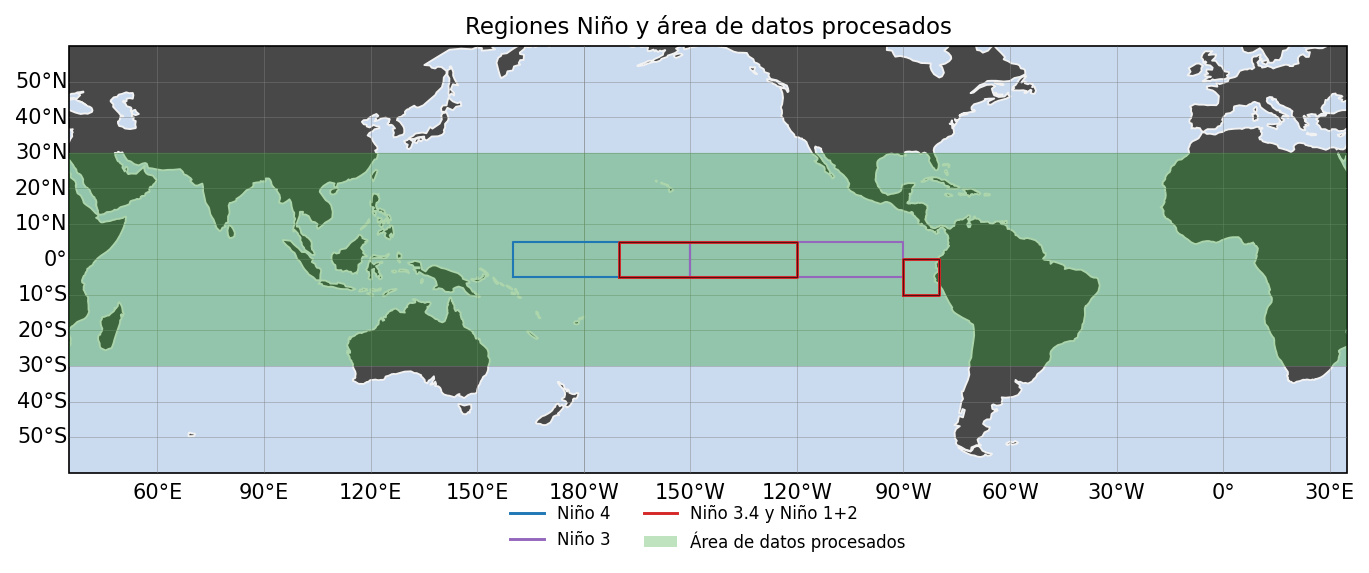
\includegraphics[width=0.9\textwidth]{figuras/region_nino_proj.png}
\caption[Ubicación de las cajas Niño~3.4 y Niño~1+2 y de la ventana de descarga.]{Regiones Niño~3.4 y Niño~1+2 (rojo), con Niño~4 y Niño~3 como referencia, en proyección cilíndrica centrada en Niño~3.4. El área verde es la ventana de descarga (0°--360°, 30°S--30°N): el dominio descargado, regrillado y enmascarado por el \emph{pipeline}. Niño~1+2, junto a la costa peruana y a la surgencia de la Corriente de Humboldt, es la caja de mayor relevancia para el monitoreo del Niño costero \citep{takahashi2019}; Niño~3.4 es la caja de referencia internacional del Índice Oceánico de El Niño (ONI).}
\label{fig:region_nino}
\end{figure}

La ventana cubre toda la franja tropical, y no solo el Pacífico, porque dos cálculos de los entregables siguientes necesitan la TSM media tropical de las tres cuencas: el índice RONI, que expresa la anomalía de Niño~3.4 relativa al promedio tropical, y el índice de calentamiento tropical del método ToD (Sección~\ref{sec:toe_metodos}). Descargar la franja completa en esta etapa evita descargas adicionales en los entregables siguientes.

Los periodos, definidos en \texttt{config/periods.yaml}, son: referencia y validación 1981--2014; proyección 2036--2065 (P1) y 2071--2100 (P2). El rango completo de descarga es 1850--2100 (\texttt{historical}: 1850--2014; escenarios SSP: 2015--2100). Los escenarios son \texttt{ssp245} y \texttt{ssp585}, más \texttt{ssp370} como escenario intermedio para el análisis de sensibilidad entre ambos. El único criterio de selección es la disponibilidad de \texttt{tos}/\texttt{Omon} en los cuatro experimentos.

% ============================================================
\section{Arquitectura del \emph{pipeline}}
\label{sec:arquitectura}
% ============================================================

El \emph{pipeline} vive en el repositorio \archivo{smn_toe}, tiene un único punto de entrada (\texttt{run.sh}) y deja sus salidas en \texttt{data/processed/}, de donde el Entregable~2 las lee sin necesidad de conocer el detalle interno de este módulo. Se rige por tres principios:

\begin{itemize}
\item \textbf{Idempotencia.} Cada paso omite el procesamiento cuya salida ya existe, de modo que una corrida puede interrumpirse y reanudarse sin recalcular lo hecho. La excepción deliberada es el control de calidad, que se recalcula completo en cada corrida porque es barato y un resultado en caché puede quedar obsoleto.
\item \textbf{Verificación por valor y no por metadato.} Las unidades, los valores de relleno y la lista de meses se comprueban sobre los datos numéricos y no sobre los atributos declarados en los archivos. Existen archivos cuyo atributo contradice su contenido; por ejemplo, archivos que declaran grados Celsius y contienen valores en Kelvin.
\item \textbf{Cascada de fuentes con degradación explícita.} Si el nodo principal de ESGF no resuelve un modelo, se prueban automáticamente nodos alternativos y Copernicus CDS. Lo que ninguna fuente resuelve queda registrado en un reporte de estado, en lugar de fallar en silencio.
\end{itemize}

\texttt{run.sh} no contiene lógica de procesamiento propia: ejecuta los pasos 00, 00b, 01, 02, 03, 04, 05, 06 y 07 en ese orden fijo, o solo un rango de ellos, y registra la salida de cada uno en \texttt{logs/pipeline.log}. Al terminar cualquier corrida, completa o parcial, genera siempre el registro de modelos, las figuras automáticas, el reporte de estado y un paquete comprimido con los artefactos para actualizar el informe. Así, cada ejecución deja constancia verificable de qué modelos quedaron descargados, procesados o pendientes. La instalación, los argumentos de \texttt{run.sh}, los tiempos y el espacio en disco requeridos, y la interpretación de las salidas se describen en el documento de anexos que acompaña a este informe.

% ============================================================
\section{Obtención y procesamiento de los datos}
\label{sec:scripts}
% ============================================================

Para obtener los datos se consultó el índice de ESGF y se identificaron los 102 modelos que publican \texttt{tos}/\texttt{Omon}; se retuvieron los que publican los cuatro experimentos y, de cada uno, la variante de grilla más gruesa y un miembro de ensamble común a los cuatro. Los archivos se descargaron en cascada desde el nodo principal de ESGF, los nodos alternativos de la federación y, como último recurso, Copernicus CDS, y ERSSTv5 se descargó de NOAA PSL. Todos los modelos se regrillaron a la grilla de ERSSTv5, se homogeneizaron calendario y unidades (comprobando el valor numérico y no el atributo declarado), se enmascararon con la máscara océano-tierra de ERSSTv5 y se filtraron valores físicamente imposibles. Finalmente, un control de calidad verificó el rango físico de la TSM ($-2$ a 45\,°C; el límite superior considera que la franja tropical incluye mares marginales cálidos, como el mar Rojo y el golfo Pérsico, donde algunos modelos alcanzan de forma plausible entre 39 y 41\,°C hacia 2100 en SSP3-7.0 y SSP5-8.5) y la cobertura temporal de cada archivo, y solo se seleccionaron los modelos con los cuatro experimentos aprobados. La Figura~\ref{fig:flujograma} resume la secuencia. La descripción de cada paso y de sus controles se encuentra en el documento de anexos.

\begin{figure}[htbp]
\centering
\begin{tikzpicture}[
  scale=0.95, transform shape,
  box/.style={draw, rounded corners, fill=green!80!white!10, align=center, text width=4.2cm, minimum height=.8cm, font=\small},
  boxaux/.style={draw, rounded corners, dashed, fill=green!20!cyan!15, align=center, text width=2.6cm, minimum height=1.1cm, font=\small},
  edg/.style={-{Latex[length=3mm]}, thick},
  edgd/.style={-{Latex[length=3mm]}, dashed, gray!80!black},
  every node/.style={font=\small}
]
\node[box] (S00) at (0,0) {00: Entorno};
\node[box] (S00b) at (0,-1.5) {00b: Modelos candidatos};
\node[boxaux] (S00c) at (5.5,-1.5) {00c\\Verif. literatura};
\node[box] (S01) at (0,-3) {01: Catálogo ESGF};
\node[box] (S02) at (-2.6,-4.5) {02: Descarga CMIP6};
\node[box] (S03) at (3.9,-4.5) {03: Descarga ERSSTv5};
\node[box] (S02b) at (-2.6,-6) {02b: Nodos ESGF alt.};
\node[box] (S02c) at (-2.6,-7.5) {02c: Copernicus CDS};
\node[box] (S04) at (0.5,-9) {04: Grilla común};
\node[box] (S05) at (0.5,-10.5) {05: Máscara océano-tierra};
\node[box] (S06) at (0.5,-12) {06: Control de calidad};
\node[box] (S07) at (0.5,-13.5) {07: Inventario final};
\node[box] (S08) at (0.5,-15) {Registro de modelos};
\node[box] (S09) at (0.5,-16.5) {Gráficos, reporte y paquete};
\draw[edg] (S00) -- (S00b);
\draw[edgd] (S00b) -- (S00c);
\draw[edg] (S00b) -- (S01);
\draw[edg] (S01) -- (S02);
\draw[edg] (S02) -- (S02b);
\draw[edg] (S02b) -- (S02c);
\draw[edgd] (S02b) to[bend right=60] (S01);
\draw[edgd] (S02c) to[bend right=80] (S01);
\draw[edg] (S02.west) -- ++(-1.5,0) |- (S04.west);
\draw[edg] (S03) -- (S04);
\draw[edg] (S04) -- (S05);
\draw[edg] (S05) -- (S06);
\draw[edg] (S06) -- (S07);
\draw[edg] (S07) -- (S08);
\draw[edg] (S08) -- (S09);
\end{tikzpicture}
\caption[Flujograma del \emph{pipeline} del Entregable~1.]{Flujograma del \emph{pipeline}. Las flechas sólidas siguen la secuencia automática de \texttt{run.sh}: buscar los modelos (00b, 01), descargar (02, 03), homogeneizar (04, 05) y verificar (06, 07). Las punteadas indican el diagnóstico manual 00c y la actualización del catálogo cuando un modelo se obtiene de una fuente alternativa (02b, 02c). Las dos últimas cajas se ejecutan en cada corrida.}
\label{fig:flujograma}
\end{figure}

% ============================================================
\section{Resultados del Entregable~1}
\label{sec:resultados}
% ============================================================

Del universo de 102 modelos CMIP6 que publican \texttt{tos}/\texttt{Omon} en ESGF, 40 completaron los cuatro experimentos requeridos y aprobaron el control de calidad final: 160 combinaciones modelo-experimento, todas con estado \texttt{PASS}. El Cuadro~\ref{tab:cuentas} resume cómo se llega a esa cifra.

\begin{table}[htbp]
\centering
\caption{Del universo de modelos candidatos al conjunto seleccionado.}
\label{tab:cuentas}
\small
\begin{tabular}{@{}L{9.6cm}rL{\dimexpr\textwidth-9.6cm-1.2cm-6\tabcolsep\relax}@{}}
\toprule
\textbf{Conjunto} & \textbf{Modelos} & \textbf{Fuente} \\
\midrule
Publican \texttt{tos}/\texttt{Omon} en ESGF (universo) & 102 & Paso~00b \\
Publican \texttt{historical}, \texttt{ssp245} y \texttt{ssp585} & 49 & Paso~00b \\
Publican además \texttt{ssp370} (lista de descarga) & 41 & Paso~00b \\
Completos y aprobados en el control de calidad (seleccionados) & 40 & Pasos~06--07 \\
\midrule
Excluidos: algún experimento no disponible en ninguna fuente consultada & 44 & Pasos~00b--02 \\
Excluidos: disponibilidad o descarga incompleta & 18 & Pasos~00b--02 \\
\bottomrule
\end{tabular}
\end{table}

La Figura~\ref{fig:qc} muestra el estado de cada modelo y experimento para el universo completo. Cada celda toma uno de seis estados: aprobado (el archivo se descargó y pasó el control de calidad); rechazado (se descargó pero no lo pasó); descarga pendiente (existe un enlace de descarga activo pero el archivo aún no se descargó o procesó); sin enlace (el Paso~00b encontró el experimento, pero el Paso~01 no encontró ningún enlace activo); solo \texttt{hist-1950} (el modelo publica la variante HighResMIP 1950--2014 en lugar de \texttt{historical}; estos modelos no corren los SSP estándar y nunca reúnen los cuatro experimentos); y no disponible (el experimento no existe en ningún nodo consultado). En la corrida final no quedó ningún archivo rechazado.

\begin{figure}[htbp]
\centering
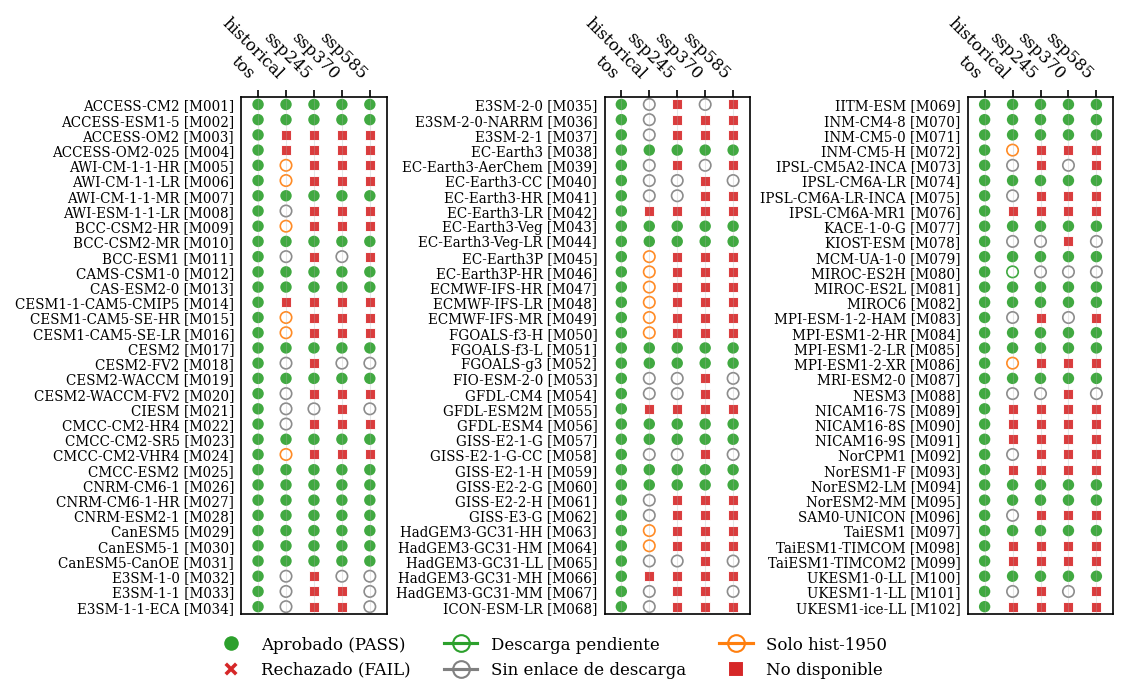
\includegraphics[width=\textwidth]{figuras/sst_QD_vf.png}
\caption[Disponibilidad y control de calidad de \texttt{tos}/\texttt{Omon} para los 102 modelos candidatos.]{Estado por modelo (nombre y código \texttt{M001}--\texttt{M102}) y por columna (\texttt{tos}, \texttt{historical}, \texttt{ssp245}, \texttt{ssp370}, \texttt{ssp585}) para los 102 modelos candidatos. Los 40 modelos seleccionados son los que tienen las cinco columnas aprobadas.}
\label{fig:qc}
\end{figure}

Como verificación exploratoria de la homogeneización, se compara ERSSTv5 con tres de los nueve modelos seleccionados de resolución nominal más gruesa, 250\,km: ACCESS-CM2, ACCESS-ESM1-5 y GISS-E2-1-G (Cuadro~\ref{tab:modelos}). Son los casos en que el regrillado a la grilla de ERSSTv5 es más exigente. Estas figuras, junto con la matriz de estado y las comparaciones por caja, las genera automáticamente \texttt{run.sh} al final de cada corrida (\archivo{scripts/plot_*.py}).

\begin{figure}[htbp]
\centering
\begin{subfigure}[t]{0.75\textwidth}
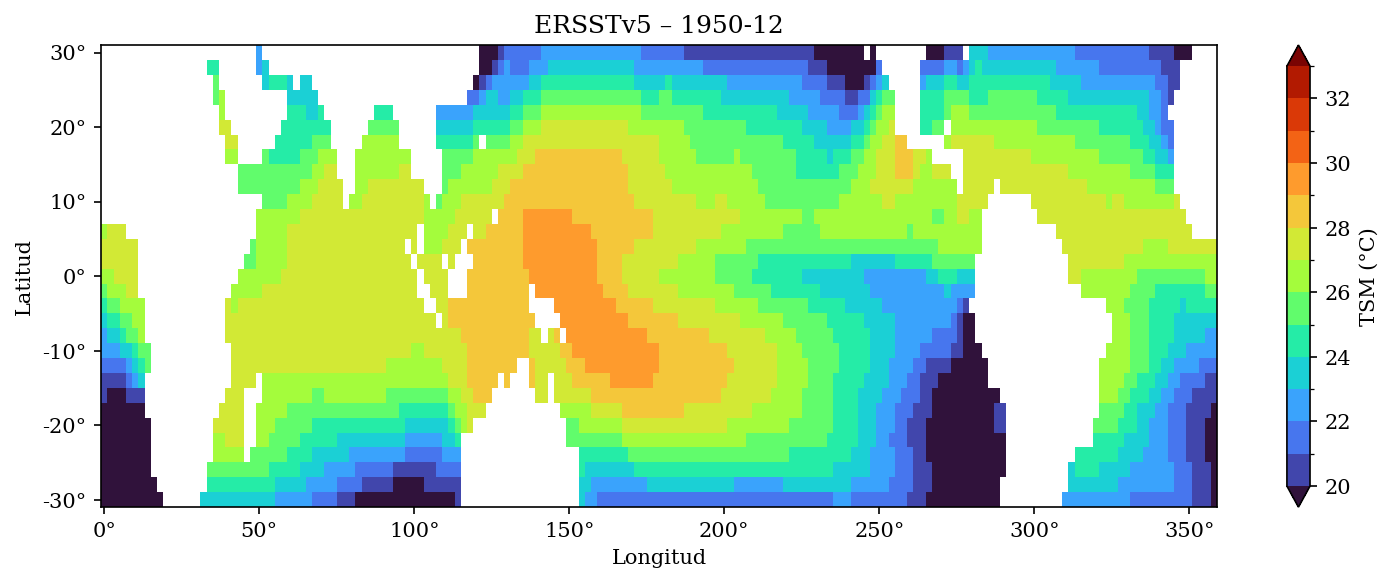
\includegraphics[width=\textwidth]{figuras/sst_2d_ERSSTv5.png}
\end{subfigure}
\begin{subfigure}[t]{0.75\textwidth}
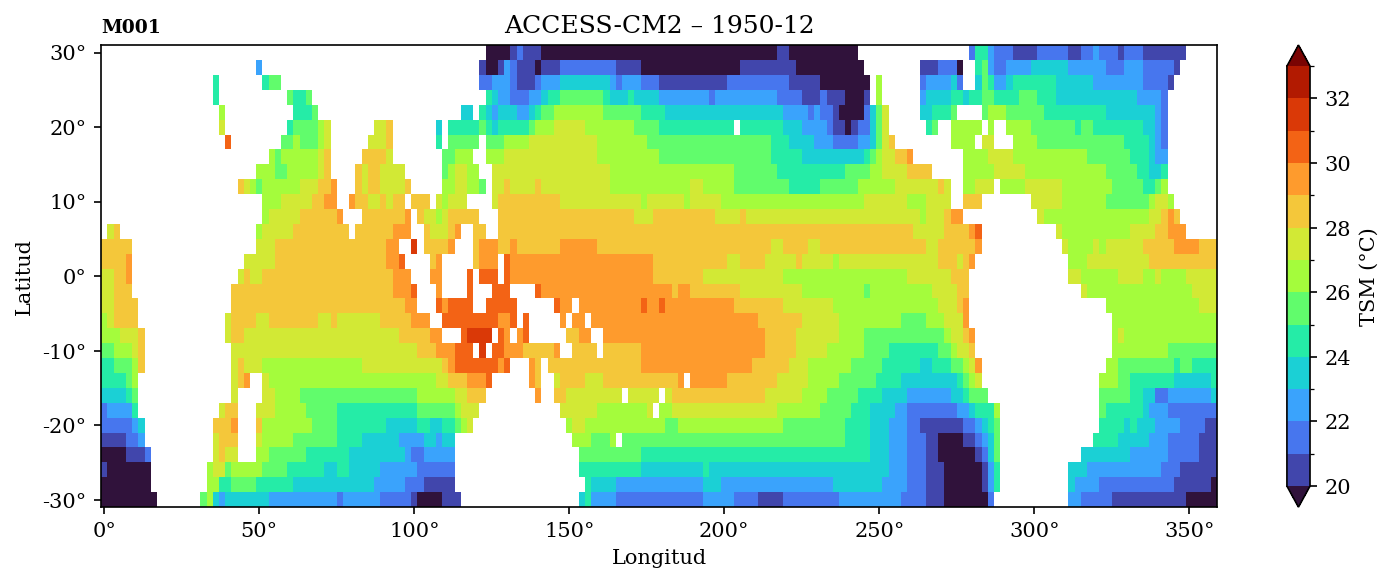
\includegraphics[width=\textwidth]{figuras/M001_sst_2d_ACCESS-CM2.png}
\end{subfigure}
\begin{subfigure}[t]{0.75\textwidth}
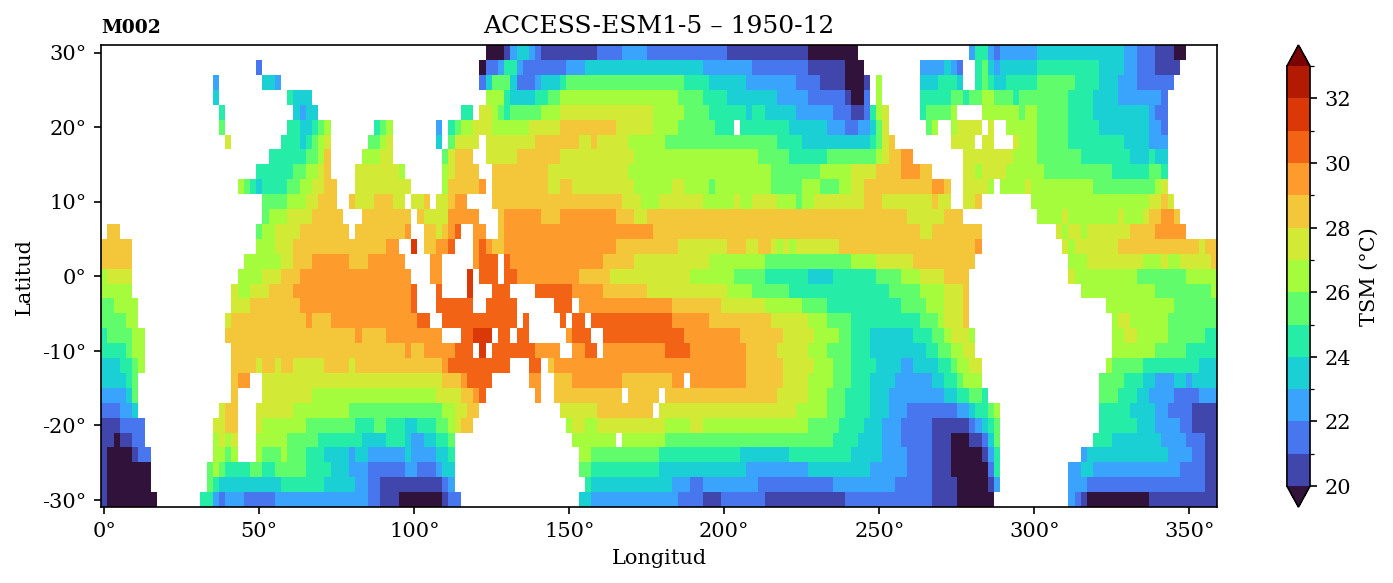
\includegraphics[width=\textwidth]{figuras/M002_sst_2d_ACCESS-ESM1-5.png}
\end{subfigure}
\begin{subfigure}[t]{0.75\textwidth}
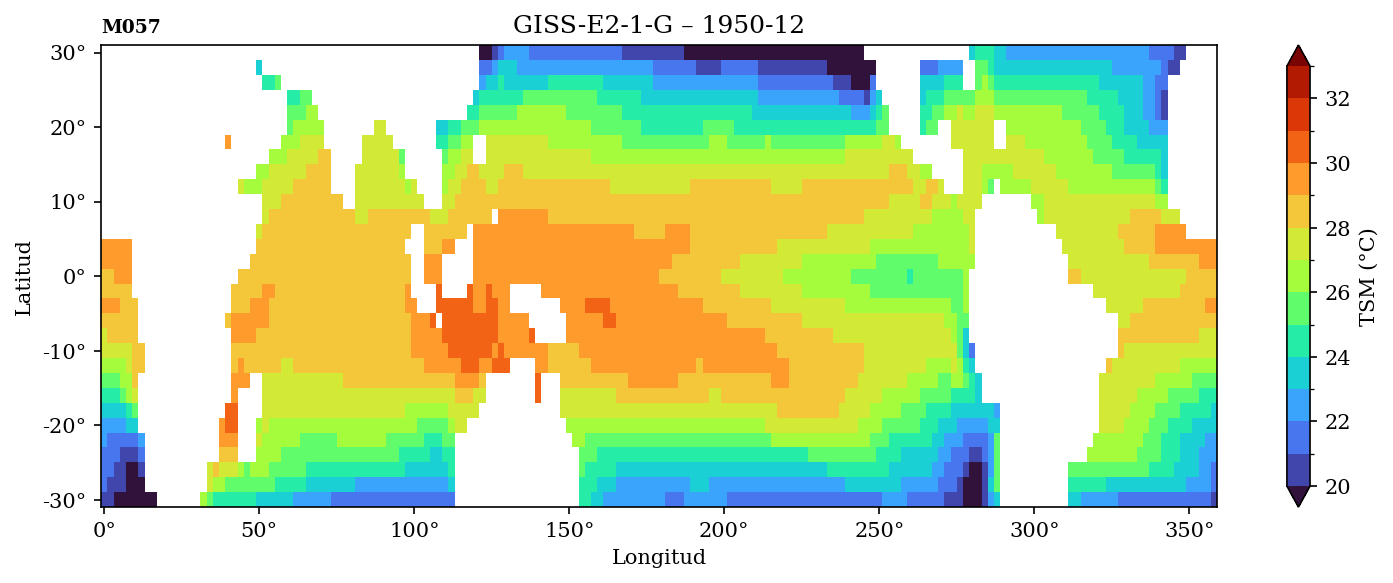
\includegraphics[width=\textwidth]{figuras/M057_sst_2d_GISS-E2-1-G.png}
\end{subfigure}
\caption[Campo de TSM de diciembre de 1950: ERSSTv5 y tres modelos de 250\,km.]{Temperatura superficial del mar de un mes de muestra (diciembre de 1950) en toda la ventana de descarga (0°--360°, 30°S--30°N), ya en la grilla, calendario, unidades y máscara océano-tierra comunes (Pasos~04--05). De arriba hacia abajo: ERSSTv5 y los modelos M001, M002 y M057 (Cuadro~\ref{tab:modelos}). Es una verificación visual de que todas las fuentes comparten grilla y máscara; al ser un mes aislado, no es una medida de desempeño.}
\label{fig:mapas2d}
\end{figure}

La Figura~\ref{fig:series} muestra la serie completa (\texttt{historical} y los tres escenarios SSP) de los mismos tres modelos en Niño~3.4, y la Figura~\ref{fig:boxplot} compara la distribución de la TSM histórica de ERSSTv5 y de los 40 modelos en ambas cajas.

\begin{figure}[htbp]
\centering
\begin{subfigure}[t]{\textwidth}
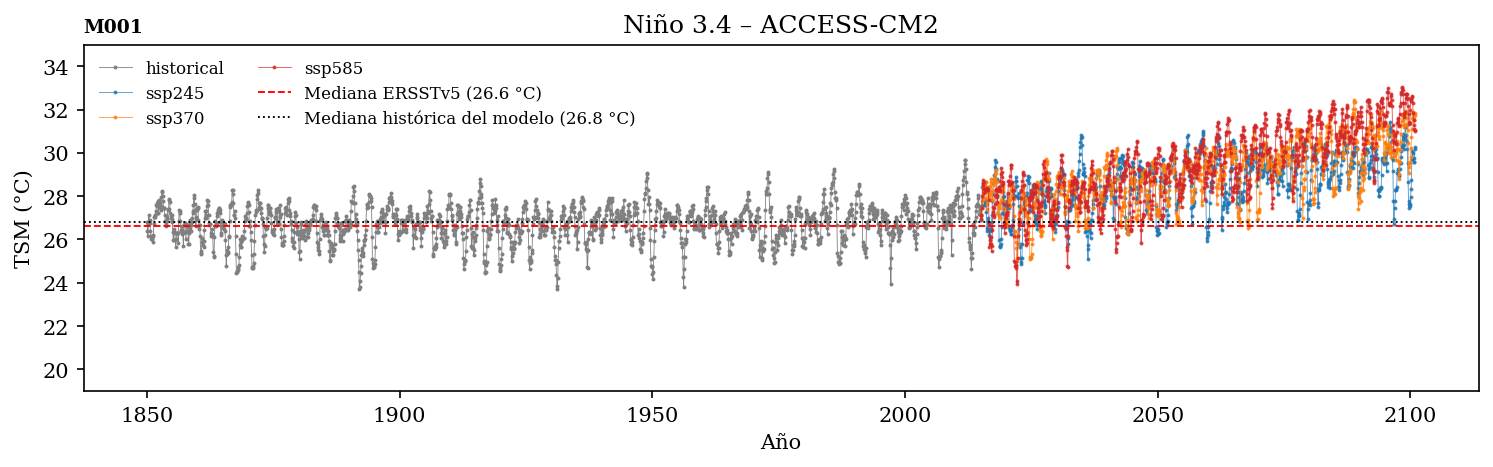
\includegraphics[width=\textwidth]{figuras/M001_serie_ACCESS-CM2_sst_Nino3.4.png}
\end{subfigure}
\begin{subfigure}[t]{\textwidth}
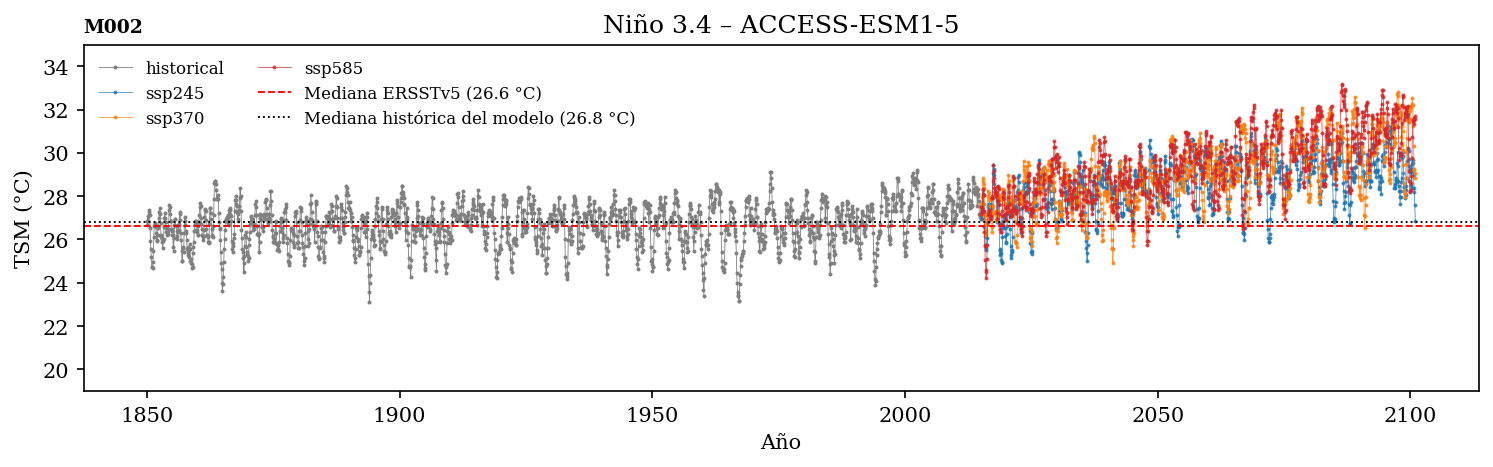
\includegraphics[width=\textwidth]{figuras/M002_serie_ACCESS-ESM1-5_sst_Nino3.4.png}
\end{subfigure}
\begin{subfigure}[t]{\textwidth}
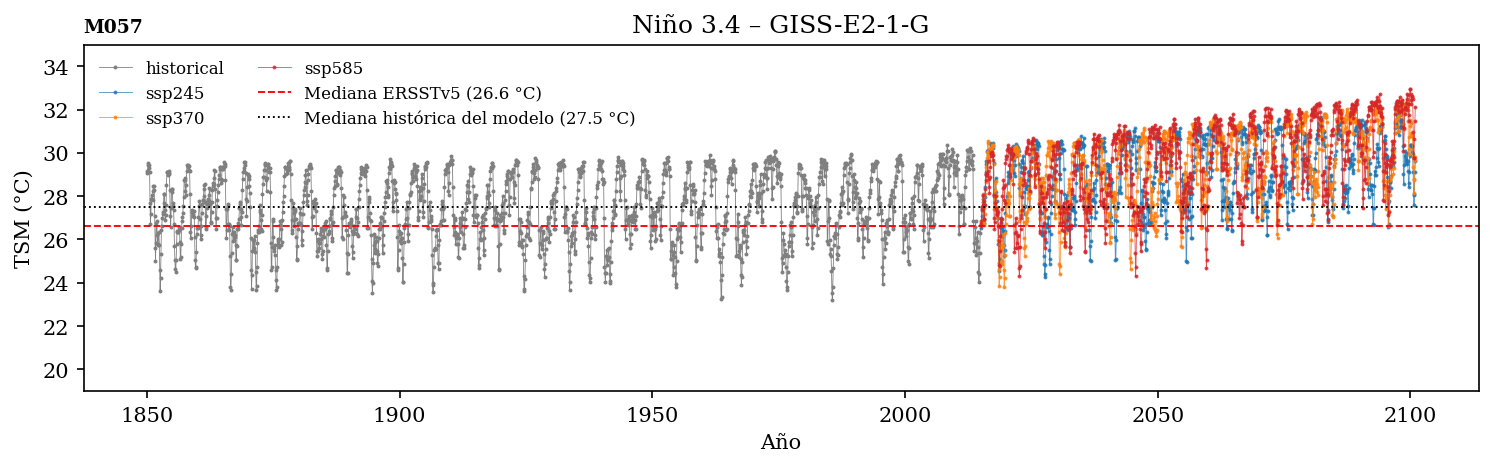
\includegraphics[width=\textwidth]{figuras/M057_serie_GISS-E2-1-G_sst_Nino3.4.png}
\end{subfigure}
\caption[Series de TSM en Niño~3.4 de tres modelos de 250\,km.]{TSM mensual promediada en Niño~3.4 (1850--2100): \texttt{historical} en gris y los tres escenarios SSP superpuestos, para los tres modelos de la Figura~\ref{fig:mapas2d}. Cada dato mensual se marca con un punto, sin interpolar huecos, de modo que un tramo sin puntos revelaría un hueco real de datos. Las líneas horizontales son la mediana de ERSSTv5 (roja, discontinua) y la mediana histórica del modelo (negra, punteada), ambas sobre el periodo común a las dos fuentes; su separación es el sesgo del modelo. El eje vertical es el mismo (19--35\,°C) en todos los paneles y en ambas cajas. Las series de Niño~1+2 se generan de la misma forma y se entregan junto con las demás figuras.}
\label{fig:series}
\end{figure}

\begin{figure}[htbp]
\centering
\begin{subfigure}[t]{\textwidth}
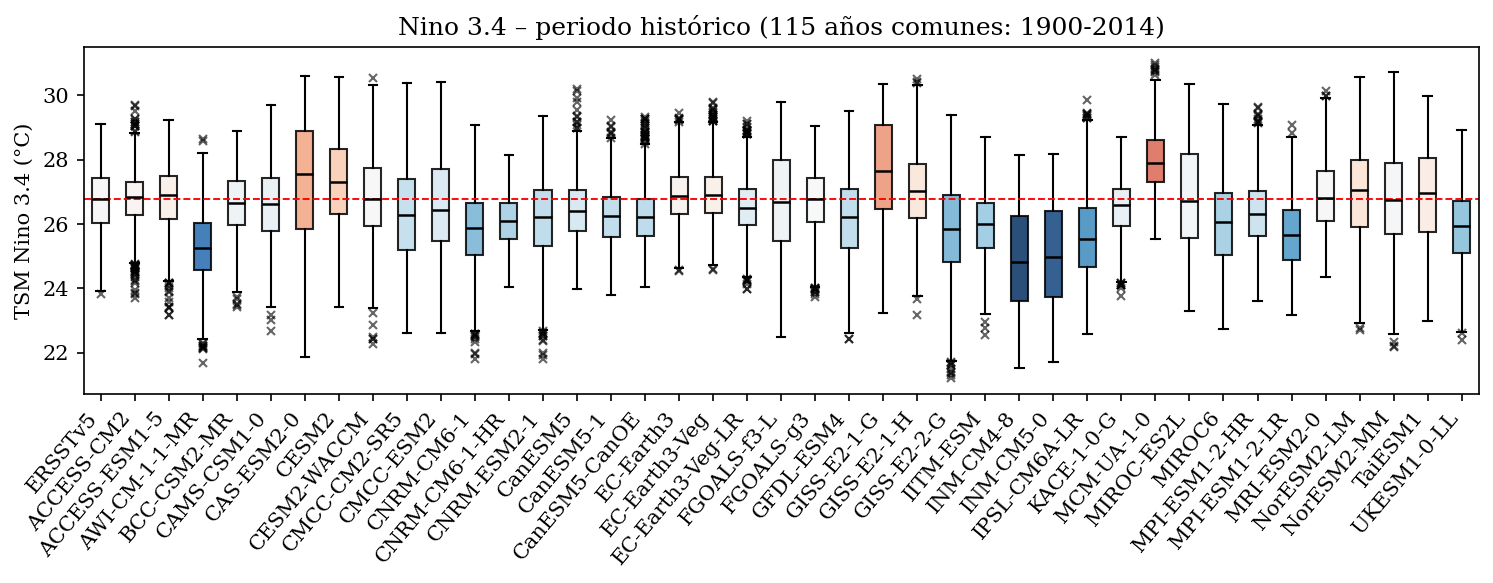
\includegraphics[width=\textwidth]{figuras/boxplot_Nino3.4.png}
\caption{Niño~3.4}
\end{subfigure}
\begin{subfigure}[t]{\textwidth}
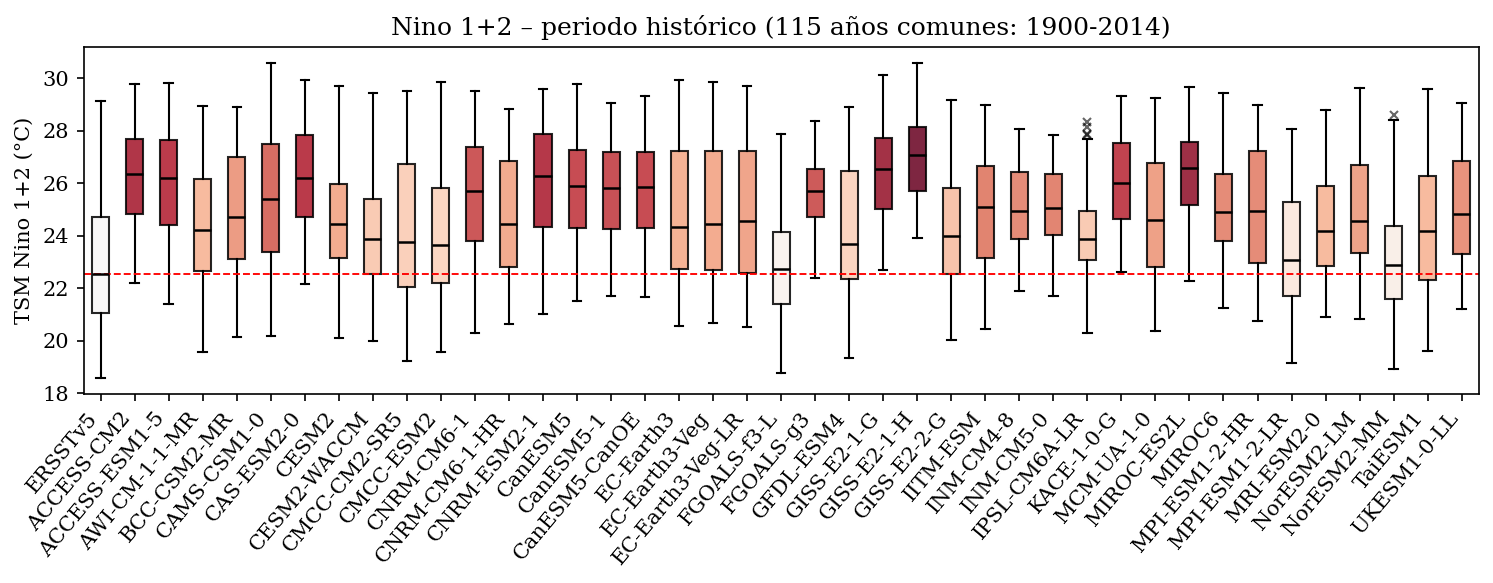
\includegraphics[width=\textwidth]{figuras/boxplot_Nino1+2.png}
\caption{Niño~1+2}
\end{subfigure}
\caption[Distribución de la TSM histórica en Niño~3.4 y Niño~1+2: ERSSTv5 frente a los 40 modelos.]{Distribución de la TSM mensual en cada caja para ERSSTv5 y los 40 modelos seleccionados, en el periodo común a todas las fuentes (1900--2014). Cada caja se colorea según la diferencia entre su mediana y la de ERSSTv5 (rojo, más cálido; azul, más frío); la línea roja discontinua marca la mediana observada.}
\label{fig:boxplot}
\end{figure}

Esta comparación preliminar ya anticipa un contraste entre cajas que el Entregable~2 deberá cuantificar. En Niño~3.4 la mediana de los modelos está cerca de la observada: 20 de los 40 modelos quedan a menos de 0{,}5\,°C de ERSSTv5 y el sesgo mediano es de $-0{,}24$\,°C. En Niño~1+2, 38 de los 40 modelos son más cálidos que la observación en más de 0{,}5\,°C, con un sesgo mediano de $+2{,}2$\,°C (rango de $+0{,}2$ a $+4{,}5$\,°C). Este sesgo cálido junto a la costa es coherente con lo señalado en la Sección~\ref{sec:similitudes} y con \citet{erickson2023}, quienes encuentran en la mayoría de los modelos CMIP6 un estado medio sesgado hacia condiciones de tipo El Niño, debido a sesgos cálidos de la TSM en el Pacífico tropical oriental. Refuerza la necesidad de reportar el sesgo de forma explícita y de calcular los índices como anomalías respecto de la climatología propia de cada modelo, de modo que el sesgo medio no se confunda con la variabilidad. La evaluación formal de desempeño (climatología, sesgos, diagrama de Taylor, índices ONI, RONI e ICEN) corresponde al Entregable~2.

\clearpage
% ============================================================
\section{Próximos pasos}
\label{sec:roadmap}
% ============================================================

El Cuadro~\ref{tab:roadmap} resume, para dar continuidad al proyecto, los análisis previstos en los Entregables~2 a~4 según las actividades~(b) a~(e) del TdR.

\begin{table}[htbp]
\caption{Análisis previstos para los Entregables~2 a~4.}
\label{tab:roadmap}
\small
\begin{tabular}{@{}L{2.2cm}L{\dimexpr\textwidth-2.2cm-2\tabcolsep\relax}@{}}
\toprule
\textbf{Entregable} & \textbf{Análisis previstos} \\
\midrule
E2 & Climatología y ciclo anual observados y simulados; sesgo, RMSE, correlación y diagrama de Taylor en ambas cajas; variabilidad interanual; eventos cálidos extremos del ENOS con ONI y RONI (Niño~3.4) e ICEN (Niño~1+2), con análisis compuesto del evento típico; puntaje de habilidad para seleccionar los modelos que mejor representan el periodo histórico. \\
E3 & Proyección del estado medio y de la variabilidad de la TSM en Niño~3.4 y Niño~1+2 bajo SSP2-4.5 y SSP5-8.5 (con SSP3-7.0 como escenario intermedio), para 2036--2065 y 2071--2100; cambios en la ocurrencia de eventos extremos del ENOS mediante ONI e ICEN. \\
E4 & Partición de la incertidumbre (variabilidad interna, modelo y escenario) y razón señal-ruido; TOE por los métodos M1 y ToD en ambas cajas; estudio técnico final con documentación metodológica, bases de datos, \emph{scripts}, conclusiones y recomendaciones, incluida la contrastación de la hipótesis de la Sección~\ref{sec:similitudes}. \\
\bottomrule
\end{tabular}
\end{table}

El Entregable~2 puede comenzar leyendo solo \texttt{data/processed/}, sin volver a ejecutar ni conocer el detalle interno de este módulo.

% ============================================================
\section{Conclusiones}
\label{sec:conclusiones}
% ============================================================

El Entregable~1, en cumplimiento de la actividad~(a) del TdR, deja construido, verificado y versionado el insumo del que dependen los Entregables~2 a~4. De su ejecución se desprenden las siguientes conclusiones:

\begin{enumerate}[label=(\roman*)]
\item El \emph{pipeline} está completo y verificado: 40 modelos CMIP6 con sus cuatro experimentos aprobados (Sección~\ref{sec:resultados}). Sus controles por valor numérico detectan problemas de los datos de origen que un control basado solo en metadatos no detectaría, como la contaminación numérica de FGOALS-f3-L y las unidades mal declaradas de GISS-E2-1-G.

\item La revisión científica (Sección~\ref{sec:marco}) sustenta la adopción de dos métodos de TOE conceptualmente independientes, M1 \citep{szabo2016} y ToD \citep{gopika2024}, y fija sus ecuaciones antes de su aplicación en el Entregable~4. De esa revisión surge además una hipótesis de trabajo contrastable: Niño~1+2 emergerá más tarde, o con mayor incertidumbre, que Niño~3.4. La mayor variabilidad interanual observada en Niño~1+2 es coherente con ella.

\item La comparación preliminar con ERSSTv5 muestra un sesgo cálido en Niño~1+2 en 38 de los 40 modelos (mediana de $+2{,}2$\,°C), mientras que en Niño~3.4 los modelos se distribuyen alrededor de la observación. La evaluación formal del Entregable~2 debe tratar ambas cajas por separado.

\item Ampliar el universo de candidatos más allá de la selección de \citet{bruno2023} deja al Entregable~2 con más información: la decisión sobre qué modelos representan mejor el ENOS se tomará con evaluación propia y no con una lista pensada para otras variables.

\item El trabajo es reproducible: el repositorio \archivo{smn_toe} es de libre acceso y, con el entorno instalado, \texttt{./run.sh} reconstruye el conjunto de datos documentado; cada corrida deja además un reporte de estado verificable. El procedimiento se detalla en el documento de anexos.
\end{enumerate}

% ============================================================
\section{Recomendaciones}
\label{sec:recomendaciones}
% ============================================================

Para la continuidad del proyecto se recomienda:

\begin{itemize}
\item Evaluar en el Entregable~2 la representación del ENOS en los 40 modelos (climatología, sesgos, métricas estadísticas e índices ONI, RONI e ICEN en ambas cajas) antes de dar por buena su idoneidad. El control de calidad de este entregable verifica la integridad y homogeneidad del dato, no su desempeño climático.
\item Verificar que la selección final de modelos del Entregable~2 conserve la dispersión estructural del ensamble \citep{lois2026}, para no subestimar la incertidumbre de modelo ni el rango del TOE.
\item Considerar la incorporación de los 8 modelos que publican \texttt{historical}, \texttt{ssp245} y \texttt{ssp585} pero no \texttt{ssp370} en los análisis que usan solo SSP2-4.5 y SSP5-8.5, lo que ampliaría los candidatos de 41 a 49 modelos.
\item Calcular y reportar M1 y ToD siempre en paralelo, documentando en el Entregable~4 los casos en que difieran sustancialmente: la bibliografía revisada muestra que esa discrepancia entre métodos es la norma y no la excepción.
\end{itemize}


\clearpage
\bibliographystyle{plainnat}
\bibliography{references_rev}

\end{document}
